\documentclass[letterpaper]{article}
\usepackage[utf8]{inputenc}
\usepackage{amsmath}
\usepackage{amsfonts}
\usepackage{amssymb}
\usepackage{graphicx}
\usepackage[left=1.00in, right=1.00in, top=1.00in, bottom=1.00in]{geometry}

\usepackage{parskip}
\usepackage{enumitem}
\usepackage[table]{xcolor}
\usepackage{siunitx}

\usepackage[T1]{fontenc}
\usepackage[scaled=1.0]{DejaVuSansMono}
\usepackage{listings}

\definecolor{codegreen}{rgb}{0,0.6,0}
\definecolor{codegray}{rgb}{0.5,0.5,0.5}
\definecolor{codepurple}{rgb}{0.58,0,0.82}
\definecolor{backcolour}{rgb}{0.965,0.973,0.980}
\lstdefinestyle{Default-Custom-Style}{
	backgroundcolor=\color{backcolour}, 
	xleftmargin=0.5cm,
	frame=tlbr,
	framesep=8pt,
	framerule=0pt,  
	%commentstyle=\color{codegreen},
	%keywordstyle=\color{magenta},
	%numberstyle=\tiny\color{codegray},
	%stringstyle=\color{codepurple},
	basicstyle=\footnotesize\ttfamily,
	breakatwhitespace=false,         
	breaklines=true,                 
	captionpos=b,                    
	keepspaces=true,                 
	numbers=none,                    
	numbersep=5pt,                  
	showspaces=false,                
	showstringspaces=false,
	showtabs=false,                  
	tabsize=2
}
\lstset{style=Default-Custom-Style}

\author{Jacob Huesman}
\title{Using difference equations to analyze a financial problem}
\begin{document}
\maketitle


\section{Introduction}
Like differential equations, difference equations can be used to model the behavior of a system. The main difference between the two being that differential equations are used to describe continuous time systems and difference equations are used to describe discrete time systems. Like the Laplace transform of a differential equation, the z-transform of a difference equation can be used to simplify solving a linear time-invariant system. This is very useful, as digital systems represent information in a discrete fashion, and there's also systems that are easier to model in discrete steps rather than as a continuous function.

This report will present an example of the application of the z-transform in modeling and solving a financial problem. The problem has been adapted from a problem posed by Dr. Green in his Signals and Systems class.

\section{Problem}
Suppose you would like to retire with 10 million dollars in savings. To keep the difference equations simple, let's say that you invest uniform monthly payments for a fixed number of years and that you receive a fixed annual percent yield. Let the interest be compounded monthly. Solve this problem with z-transform techniques for three different interest rates (low, medium, high), over three different time intervals (short, average, long). For each interest rate and investment duration, compute the required (fixed) monthly payments $C_{i,D}$ needed to realize the 10 million dollar retirement goal.

\section{Solution}
\subsection{Interest Rate and Duration}
We start by picking three realistic annual percentage rates reflective of different investments:
\begin{align*}
	i_{low}  &= \SI{0.5}{\%}  \\
	i_{med}  &= \SI{0.6}{\%}  \\
	i_{high} &= \SI{10.5}{\%}
\end{align*}

We define our investment time intervals as:
\begin{align*}
	D_{short} &= \SI{16}{years}  \\
	D_{med}   &= \SI{32}{years}  \\
	D_{long}  &= \SI{48}{years}
\end{align*}

\pagebreak
\subsection{Difference Equation}
Let $n=0$ correspond to the first investment contribution, let $n = 12D -1$ be the last investment contribution, and let $n = 12D$ be the time when the retirement account is to have the desired 10 million dollars in savings. Our difference equation is then
\begin{align}
	y[n] &= \left(1 + \frac{i}{100} \right)^{\frac{1}{12}} y[n-1] + C (u[n] - u[n-12D]). \label{eq1}
\end{align}
where $y[n]$ is the balance at month $n$, $\left(1 + \frac{i}{100} \right)^{\frac{1}{12}} y[n-1]$ is last month's balance plus the accrued interest, and $C(u[n] - u[n-12D])$ is the payments made each month over the specified duration. For the payments made each month, we had to include some unit step functions to handle the last month where no payment is made, but interest is still accrued.

\subsection{Z-Transform}

Now putting equation \ref{eq1} in standard form and simplifying we get,
\begin{align}
	y[n] - \left(1 + \frac{i}{100} \right)^{\frac{1}{12}} y[n-1] &= C (u[n] - u[n-12D]) \\
	\left(1 - \left(1 + \frac{i}{100} \right)^{\frac{1}{12}}E^{-1}\right)y[n] &= C (u[n] - u[n-12D]). \label{eq2}
\end{align}
Note that $E^{-1}$ is used to denote a delay operation. Having put equation \ref{eq1} in a more standard form we can take the z-transform of both sides.
\begin{align}
	\left(1 - \left(1 + \frac{i}{100} \right)^{\frac{1}{12}}z^{-1}\right)Y(z) &= C \left(\frac{z}{z-1} - \frac{z^{-12D+1}}{z-1} \right).
\end{align}

Which can be written as
\begin{align}
	Y(z) &=  C\left(\frac{\frac{z}{z-1} - \frac{z^{-12D+1}}{z-1}}
	{1 - \left(1 + \frac{i}{100} \right)^{\frac{1}{12}}z^{-1}}\right). \label{eq3} \\
	     &=  C\left(\frac{z - z^{-12D+1}}{(z-1)(1 - p z^{-1})}\right)
\end{align}
where 
\begin{align}
	p = \left(1 + \frac{i}{100} \right)^{\frac{1}{12}}.
\end{align}
Note that a delay in the time domain corresponds to a negative power of z in the z-domain by the time shifting property:
\begin{align}
	\text{If }m>0: x[n-m]u[n-m] \stackrel{Z_u}{\Longleftrightarrow} z^{-m} X(z) \label{prop1}
\end{align}
We also used one z-transform pair from a table:
\begin{align}
	&\gamma^nu[n] \stackrel{Z_u}{\Longleftrightarrow} \frac{z}{z-\gamma} & &\text{ROC: } |z|>|\gamma| \label{tp1}
\end{align}

\subsection{Modified Partial Fraction Expansion}
Like solving differential equations with the Laplace Transform, typically difference equations are solved by breaking the resulting equation into smaller pieces and then referencing a table of Z-Transforms to bring the equation back into the time domain. The process of breaking the equation into smaller pieces is known as the modified partial fraction expansion. It's the same the partial fraction expansion used in Laplace transforms except since most z-transform tables require a $z$ in the numerator, we pull a $z$ out of the equation before performing the expansion, then return it after the expansion is complete.

We'll simplify (\ref{eq3}) and pull out the z before performing the expansion
\begin{align}
	\frac{Y(z)}{z} &= C \left( \frac{z - z^{-12D+1}}{z(z-1)(1 - pz^{-1})} \right) \\
	&= C \left( \frac{z - z^{-12D+1}}{(z-1)(z - p)} \right).
\end{align}
Let
\begin{align}
	\frac{Y_1(z)}{z} &= \frac{z}{(z-1)(z - p)} \\
	\frac{Y_2(z)}{z} &= \frac{z^{-12D+1}}{(z-1)(z - p)}
\end{align}
then
\begin{align}
	\frac{Y(z)}{z} &= C \left( \frac{Y_1(z)}{z} - \frac{Y_2(z)}{z} \right).
\end{align}

We start by solving for $Y_1(z)$,
\begin{align}
	\frac{Y_1(z)}{z} &= \frac{z}{(z-1)(z - p)} \\
					 &= \frac{A}{z-1} + \frac{B}{z-p}
\end{align}

Using the Heaviside cover-up method
\begin{align}
	A &= \frac{1}{1 - p} \\
	B &= \frac{p}{p - 1}
\end{align}
So
\begin{align}
	\frac{Y_1(z)}{z} &= \left(\frac{1}{1 - p}\right)\left(\frac{1}{z-1}\right) 
						+ \left(\frac{p}{p - 1}\right)\left(\frac{1}{z-p}\right) 
\end{align}
Now in order to use (\ref{tp1}) we need a $z$ in the numerator of each component of the sum, so we move the $z$ on the LHS back over,
\begin{align}
	Y_1(z) &= \left(\frac{1}{1 - p}\right)\left(\frac{z}{z-1}\right) 
	+ \left(\frac{p}{p - 1}\right)\left(\frac{z}{z-p}\right).
\end{align}

\pagebreak
\subsection{Inverse Z-Transform}
Using (\ref{tp1}) we can find the inverse z-transform of $Y_1$
\begin{align}
	Z^{-1}\left[Y_1(z)\right] &= \frac{1}{1 - p}u[n] + \frac{p}{p - 1}p^n u[n] \\
							  &= \left(\frac{1}{1 - p} + \frac{p}{p - 1}p^n \right)u[n] \\
							  &= \left(\frac{1}{p - 1}p^{n+1} - \frac{1}{p - 1} \right)u[n] \\
							  &= \frac{1}{p - 1}\left(p^{n+1} - 1 \right)u[n] \\
							  &= y_1[n]
\end{align}

Having found $y_1[n]$ we can use the time shift property (\ref{prop1}) to find $y_2[n]$. First note that we originally wrote $Y_2(z)$ as
\begin{align}
	\frac{Y_2(z)}{z} &= \frac{z^{-12D+1}}{(z-1)(z - p)}.
\end{align}

However, since we have already done the modified partial fraction decomposition on $Y_1(z)$ and will be using properties to find $Y_2(z)$, we no longer need $Y_1(z)$, $Y_2(z)$, or $Y(z)$ in that form, so we write
\begin{align}
	Y_1(z) &= \frac{z^2}{(z-1)(z - p)} \\
	Y_2(z) &= \frac{z^{-12D+2}}{(z-1)(z - p)} \\
	Y(z)   &= C \left(Y_1(z) - Y_2(z) \right).
\end{align}

Notice 
\begin{align}
	Y_2(z) &= \frac{z^{-12D+2}}{(z-1)(z - p)} \\
	       &= \frac{z^{2}}{(z-1)(z - p)}z^{-12D} \\
	       &= Y_1(z) z^{-12D}
\end{align}

We can use the time shift property (\ref{prop1}) to find 
\begin{align}
	Z^{-1}\left[Y_2\right] &= Z^{-1}\left[Y_1(z) z^{-12D}\right] \\
						   &= \frac{1}{p - 1}\left(p^{n+1-12D} - 1 \right)u[n-12D] \\
						   &= y_2[n]
\end{align}

Having found both $y_1[n]$ and $y_2[n]$ we can use Linearity to find $y[n]$. The z-transform is a linear transformation, so 
\begin{align}
	ax[n] + by[n] \stackrel{Z_u}{\Longleftrightarrow} aX(z) + bY(z) \label{prop2}
\end{align}

Which means that 
\begin{align}
	C \left(Y_1(z) - Y_2(z) \right) &\stackrel{Z_u}{\Longleftrightarrow} C \left(y_1[n] - y_2[n] \right) \\
	Y(z) &\stackrel{Z_u}{\Longleftrightarrow} y[n]
\end{align}

So using (\ref{prop2})
\begin{align}
	y[n] &= C(y_1[n] - y_2[n]) \\
		 &= C \left(\frac{1}{p - 1}\left(p^{n+1} - 1 \right)u[n] - \frac{1}{p - 1}\left(p^{n+1-12D} - 1 \right)u[n-12D] \right) \\
		 &= \frac{C}{p - 1}\left(\left(p^{n+1} - 1 \right)u[n] - \left(p^{n+1-12D} - 1 \right)u[n-12D] \right). \label{eqny}
\end{align}

We now have a solution to our investment problem for an arbitrary monthly payment amount, interest, and investment duration. A pretty cool application of the z-transform. 

\subsection{Monthly payments}
Equation (\ref{eqny}) is useful if we want to see what our projected balance would be on a given month. However we are interested in our monthly payments, given a goal, interest, and duration. So we'll rearrange (\ref{eqny}) as
\begin{align}
	C &= \frac{y[n](p - 1)}{\left(p^{n+1} - 1 \right)u[n] - \left(p^{n+1-12D} - 1 			\right)u[n-12D]} \\
	  &= \frac{y[12D](p - 1)}{\left(p^{12D+1} - 1 \right)u[12D] - \left(p^{12D+1-12D} - 1 \right)u[12D-12D]} \\
	  &= \frac{\SI{10}{M}(p - 1)}{p^{12D+1} - 1 - p^1 + 1} \\
	  &= \frac{\SI{10}{M}(p - 1)}{p\left(p^{12D} - 1\right)}
\end{align}

Having solved for $C$ we use MATLAB to find $C_{i,D}$ given our three interests and durations
\begin{table}[h]
	\centering
	\begin{tabular}{|r|r|r|r|}
		\hline 
		D, i & 0.5\% & 6\% & 10.5\% \\ 
		\hline 
		16 years & \$50,022.43 & \$31,447.18 & \$21,026.04 \\ 
		\hline 
		32 years & \$24,013.78 & \$8,882.5 & \$3,539.26 \\ 
		\hline 
		48 years & \$15,362.61 & \$3,146.68 & \$692.73 \\ 
		\hline 
	\end{tabular} 
	\caption[Table 1:]{Monthly contribution for particular APYs and investment durations}
\end{table}

\pagebreak
\subsection{Investment Growth}
Looking at the investment growth with different APYs and investment durations shows pretty clearly that of the two factors we have some control over, duration is the more important one, it also happens to be the one we have the most control over. 
\begin{center}
	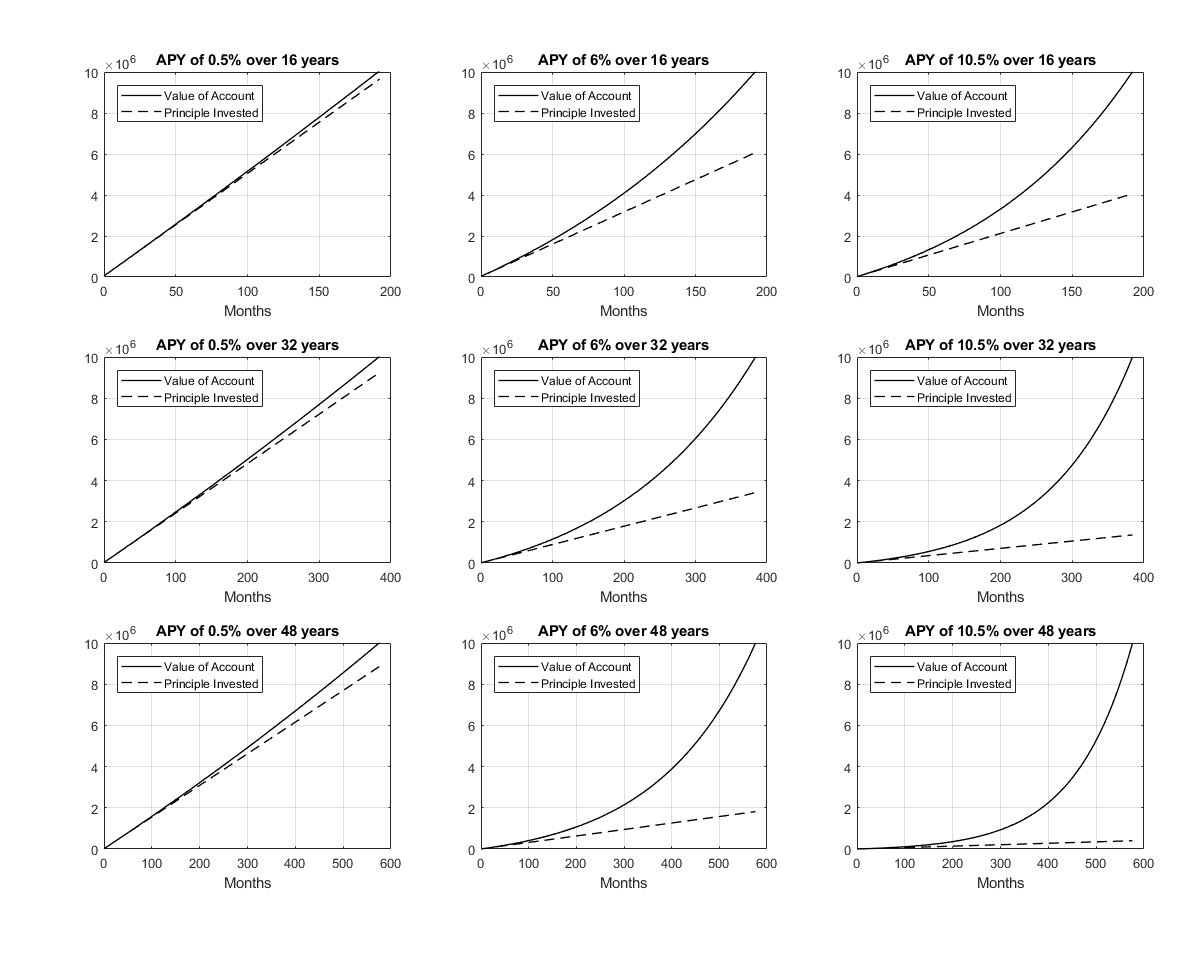
\includegraphics[width=1\linewidth]{../matlab/investment_growth.png}
\end{center}


\section{Conclusion}
This  was a fairly simple example, but the techniques demonstrated here can be used to solve much more complex financial problems. You just need to be able to write it out as a difference equation and employ the techniques demonstrated above.

Handling finances intelligently is important for long term success. Although using the z-transform is not the only way, or really even an obvious way, it's a fairly simple tool that can be employed to quickly solve a financial problem. 

\pagebreak
\section{Appendix}
\subsection{MATLAB Code}
\begin{lstlisting}[language=MATLAB]
clear;

i = [0.5, 6.0, 10.5];
D = [16, 32, 48];
Y_r = 10E6;

p = (1 + i./100).^(1/12);

C = (Y_r .* (p - 1)) ./ (p .* (p.^(12.*D') - 1));
P = 12.*D'.*C;

u = @(t) 1.0 .* (t >= 0);
y = @(n, C, p, D) C ./ (p - 1) .* ( (p.^(n + 1) - 1).*u(n) - (p.^(n + 1 - 12*D) - 1).*u(n - 12*D));
for j = 1:1:3
	n = 0:1:(D(j)*12);
	P_t = (n+1) .* C(j,:)';
	y_t = y(n, C(j,:)', p', D(j));
	for k = 1:1:3     
		subplot(3,3,((j-1)*3+k-1)+1);
		plot(n, y_t(k,:), '-', n, P_t(k,:), '--', 'color', [0,0,0], 'linewidth', 1);
		title("APY of " + string(i(k))+"% over " + string(D(j)) + " years");
		legend('Value of Account', 'Principle Invested', 'Location','northwest');
		xlabel('Months');
		grid on;
	end
end
\end{lstlisting}


\end{document}